\documentclass[twoside]{book}

% Packages required by doxygen
\usepackage{fixltx2e}
\usepackage{calc}
\usepackage{doxygen}
\usepackage[export]{adjustbox} % also loads graphicx
\usepackage{graphicx}
\usepackage[utf8]{inputenc}
\usepackage{makeidx}
\usepackage{multicol}
\usepackage{multirow}
\PassOptionsToPackage{warn}{textcomp}
\usepackage{textcomp}
\usepackage[nointegrals]{wasysym}
\usepackage[table]{xcolor}

% Font selection
\usepackage[T1]{fontenc}
\usepackage[scaled=.90]{helvet}
\usepackage{courier}
\usepackage{amssymb}
\usepackage{sectsty}
\renewcommand{\familydefault}{\sfdefault}
\allsectionsfont{%
  \fontseries{bc}\selectfont%
  \color{darkgray}%
}
\renewcommand{\DoxyLabelFont}{%
  \fontseries{bc}\selectfont%
  \color{darkgray}%
}
\newcommand{\+}{\discretionary{\mbox{\scriptsize$\hookleftarrow$}}{}{}}

% Page & text layout
\usepackage{geometry}
\geometry{%
  a4paper,%
  top=2.5cm,%
  bottom=2.5cm,%
  left=2.5cm,%
  right=2.5cm%
}
\tolerance=750
\hfuzz=15pt
\hbadness=750
\setlength{\emergencystretch}{15pt}
\setlength{\parindent}{0cm}
\setlength{\parskip}{3ex plus 2ex minus 2ex}
\makeatletter
\renewcommand{\paragraph}{%
  \@startsection{paragraph}{4}{0ex}{-1.0ex}{1.0ex}{%
    \normalfont\normalsize\bfseries\SS@parafont%
  }%
}
\renewcommand{\subparagraph}{%
  \@startsection{subparagraph}{5}{0ex}{-1.0ex}{1.0ex}{%
    \normalfont\normalsize\bfseries\SS@subparafont%
  }%
}
\makeatother

% Headers & footers
\usepackage{fancyhdr}
\pagestyle{fancyplain}
\fancyhead[LE]{\fancyplain{}{\bfseries\thepage}}
\fancyhead[CE]{\fancyplain{}{}}
\fancyhead[RE]{\fancyplain{}{\bfseries\leftmark}}
\fancyhead[LO]{\fancyplain{}{\bfseries\rightmark}}
\fancyhead[CO]{\fancyplain{}{}}
\fancyhead[RO]{\fancyplain{}{\bfseries\thepage}}
\fancyfoot[LE]{\fancyplain{}{}}
\fancyfoot[CE]{\fancyplain{}{}}
\fancyfoot[RE]{\fancyplain{}{\bfseries\scriptsize Generated by Doxygen }}
\fancyfoot[LO]{\fancyplain{}{\bfseries\scriptsize Generated by Doxygen }}
\fancyfoot[CO]{\fancyplain{}{}}
\fancyfoot[RO]{\fancyplain{}{}}
\renewcommand{\footrulewidth}{0.4pt}
\renewcommand{\chaptermark}[1]{%
  \markboth{#1}{}%
}
\renewcommand{\sectionmark}[1]{%
  \markright{\thesection\ #1}%
}

% Indices & bibliography
\usepackage{natbib}
\usepackage[titles]{tocloft}
\setcounter{tocdepth}{3}
\setcounter{secnumdepth}{5}
\makeindex

% Hyperlinks (required, but should be loaded last)
\usepackage{ifpdf}
\ifpdf
  \usepackage[pdftex,pagebackref=true]{hyperref}
\else
  \usepackage[ps2pdf,pagebackref=true]{hyperref}
\fi
\hypersetup{%
  colorlinks=true,%
  linkcolor=blue,%
  citecolor=blue,%
  unicode%
}

% Custom commands
\newcommand{\clearemptydoublepage}{%
  \newpage{\pagestyle{empty}\cleardoublepage}%
}

\usepackage{caption}
\captionsetup{labelsep=space,justification=centering,font={bf},singlelinecheck=off,skip=4pt,position=top}

%===== C O N T E N T S =====

\begin{document}

% Titlepage & ToC
\hypersetup{pageanchor=false,
             bookmarksnumbered=true,
             pdfencoding=unicode
            }
\pagenumbering{alph}
\begin{titlepage}
\vspace*{7cm}
\begin{center}%
{\Large Spannungsteiler-\/\+Berechnungstool }\\
\vspace*{1cm}
{\large Generated by Doxygen 1.8.13}\\
\end{center}
\end{titlepage}
\clearemptydoublepage
\pagenumbering{roman}
\tableofcontents
\clearemptydoublepage
\pagenumbering{arabic}
\hypersetup{pageanchor=true}

%--- Begin generated contents ---
\chapter{Spannungsteiler-\/\+Berechnungstool}
\label{index}\hypertarget{index}{}\doxysection*{Project description}

G\+UI to calculate the ideal resistor-\/ratio of a simple unloaded voltage divider. 
\chapter{Hierarchical Index}
\doxysection{Class Hierarchy}
This inheritance list is sorted roughly, but not completely, alphabetically\+:\begin{DoxyCompactList}
\item \contentsline{section}{evaluate\+Resistor}{\pageref{classevaluateResistor}}{}
\item Q\+Main\+Window\begin{DoxyCompactList}
\item \contentsline{section}{Main\+Window}{\pageref{classMainWindow}}{}
\end{DoxyCompactList}
\item \contentsline{section}{Test}{\pageref{classTest}}{}
\end{DoxyCompactList}

\chapter{Class Index}
\section{Class List}
Here are the classes, structs, unions and interfaces with brief descriptions\+:\begin{DoxyCompactList}
\item\contentsline{section}{\hyperlink{classevaluateResistor}{evaluate\+Resistor} }{\pageref{classevaluateResistor}}{}
\item\contentsline{section}{\hyperlink{classMainWindow}{Main\+Window} \\*Qt \hyperlink{classMainWindow}{Main\+Window} Builds the G\+UI for the \char`\"{}\+Spannungsteiler-\/\+Berechnungstool\char`\"{} }{\pageref{classMainWindow}}{}
\item\contentsline{section}{\hyperlink{classTest}{Test} \\*A \hyperlink{classTest}{Test} class Includes both functions for user input check }{\pageref{classTest}}{}
\end{DoxyCompactList}

\chapter{Class Documentation}
\hypertarget{classevaluateResistor}{}\section{evaluate\+Resistor Class Reference}
\label{classevaluateResistor}\index{evaluate\+Resistor@{evaluate\+Resistor}}
\subsection*{Static Public Member Functions}
\begin{DoxyCompactItemize}
\item 
\mbox{\Hypertarget{classevaluateResistor_a0d434e47b94ce646cbcd10e6f1f2e084}\label{classevaluateResistor_a0d434e47b94ce646cbcd10e6f1f2e084}} 
static double {\bfseries find\+Closest} (double value, const double $\ast$e\+Serie)
\end{DoxyCompactItemize}
\subsection*{Static Public Attributes}
\begin{DoxyCompactItemize}
\item 
\mbox{\Hypertarget{classevaluateResistor_af5e266c489d3034f4077ca44f59a6c1d}\label{classevaluateResistor_af5e266c489d3034f4077ca44f59a6c1d}} 
static const double {\bfseries E3} \mbox{[}$\,$\mbox{]} = \{1.\+0, 2.\+2, 4.\+7, 0.\+0\}
\item 
\mbox{\Hypertarget{classevaluateResistor_a4740a0fe56c3bee3a254f3f2cb041e81}\label{classevaluateResistor_a4740a0fe56c3bee3a254f3f2cb041e81}} 
static const double {\bfseries E6} \mbox{[}$\,$\mbox{]} = \{1.\+0, 1.\+5, 2.\+2, 3.\+3, 4.\+7, 6.\+8, 0.\+0\}
\item 
static const double {\bfseries E12} \mbox{[}$\,$\mbox{]}
\item 
static const double {\bfseries E24} \mbox{[}$\,$\mbox{]}
\end{DoxyCompactItemize}


\subsection{Member Data Documentation}
\mbox{\Hypertarget{classevaluateResistor_a4ad1d14208c52720ebded7accf2ed219}\label{classevaluateResistor_a4ad1d14208c52720ebded7accf2ed219}} 
\index{evaluate\+Resistor@{evaluate\+Resistor}!E12@{E12}}
\index{E12@{E12}!evaluate\+Resistor@{evaluate\+Resistor}}
\subsubsection{\texorpdfstring{E12}{E12}}
{\footnotesize\ttfamily const double evaluate\+Resistor\+::\+E12\hspace{0.3cm}{\ttfamily [static]}}

{\bfseries Initial value\+:}
\begin{DoxyCode}
= \{1.0, 1.2, 1.5, 1.8, 2.2, 2.7, 3.3,
                                        3.9, 4.7, 5.6, 6.8, 8.2, 0.0\}
\end{DoxyCode}
\mbox{\Hypertarget{classevaluateResistor_a05152df560338e850ff81a930267b246}\label{classevaluateResistor_a05152df560338e850ff81a930267b246}} 
\index{evaluate\+Resistor@{evaluate\+Resistor}!E24@{E24}}
\index{E24@{E24}!evaluate\+Resistor@{evaluate\+Resistor}}
\subsubsection{\texorpdfstring{E24}{E24}}
{\footnotesize\ttfamily const double evaluate\+Resistor\+::\+E24\hspace{0.3cm}{\ttfamily [static]}}

{\bfseries Initial value\+:}
\begin{DoxyCode}
= \{
    1.0, 1.1, 1.2, 1.3, 1.5, 1.6, 1.8, 2.0, 2.2, 2.4, 2.7, 3.0, 3.3,
    3.6, 3.9, 4.3, 4.7, 5.1, 5.6, 6.2, 6.8, 7.5, 8.2, 9.1, 0.0\}
\end{DoxyCode}


The documentation for this class was generated from the following files\+:\begin{DoxyCompactItemize}
\item 
include/evaluate\+Resistor.\+h\item 
src/evaluate\+Resistor.\+cpp\end{DoxyCompactItemize}

\hypertarget{classMainWindow}{}\section{Main\+Window Class Reference}
\label{classMainWindow}\index{Main\+Window@{Main\+Window}}


Qt \hyperlink{classMainWindow}{Main\+Window} Builds the G\+UI for the \char`\"{}\+Spannungsteiler-\/\+Berechnungstool\char`\"{}.  




{\ttfamily \#include $<$Main\+Window.\+h$>$}



Inheritance diagram for Main\+Window\+:
\nopagebreak
\begin{figure}[H]
\begin{center}
\leavevmode
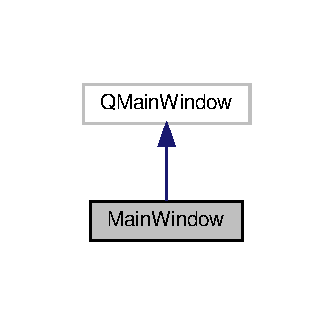
\includegraphics[width=160pt]{classMainWindow__inherit__graph}
\end{center}
\end{figure}
\subsection*{Public Member Functions}
\begin{DoxyCompactItemize}
\item 
\hyperlink{classMainWindow_a996c5a2b6f77944776856f08ec30858d}{Main\+Window} (Q\+Widget $\ast$parent=nullptr)
\begin{DoxyCompactList}\small\item\em Creates the main window object. \end{DoxyCompactList}\end{DoxyCompactItemize}


\subsection{Detailed Description}
Qt \hyperlink{classMainWindow}{Main\+Window} Builds the G\+UI for the \char`\"{}\+Spannungsteiler-\/\+Berechnungstool\char`\"{}. 

\subsection{Constructor \& Destructor Documentation}
\mbox{\Hypertarget{classMainWindow_a996c5a2b6f77944776856f08ec30858d}\label{classMainWindow_a996c5a2b6f77944776856f08ec30858d}} 
\index{Main\+Window@{Main\+Window}!Main\+Window@{Main\+Window}}
\index{Main\+Window@{Main\+Window}!Main\+Window@{Main\+Window}}
\subsubsection{\texorpdfstring{Main\+Window()}{MainWindow()}}
{\footnotesize\ttfamily Main\+Window\+::\+Main\+Window (\begin{DoxyParamCaption}\item[{Q\+Widget $\ast$}]{parent = {\ttfamily nullptr} }\end{DoxyParamCaption})\hspace{0.3cm}{\ttfamily [explicit]}}



Creates the main window object. 


\begin{DoxyParams}{Parameters}
{\em parent} & parent object \\
\hline
\end{DoxyParams}


The documentation for this class was generated from the following file\+:\begin{DoxyCompactItemize}
\item 
include/Main\+Window.\+h\end{DoxyCompactItemize}

\hypertarget{classTest}{}\section{Test Class Reference}
\label{classTest}\index{Test@{Test}}


A \hyperlink{classTest}{Test} class Includes both functions for user input check.  




{\ttfamily \#include $<$Check\+Input.\+h$>$}

\subsection*{Public Member Functions}
\begin{DoxyCompactItemize}
\item 
int \hyperlink{classTest_a3b223ab01f34445e73b914b48a2ff7fc}{check\+Inputfrom\+Keyboard} (Q\+String $\ast$str1, Q\+String $\ast$str2)
\begin{DoxyCompactList}\small\item\em Verifies the plausibility of the values entered by the user. \end{DoxyCompactList}\item 
void \hyperlink{classTest_a83a0f09e6583bf623f84f0caa50342d9}{replace\+Invalid\+Char} (Q\+String \&str1, Q\+String \&str2)
\begin{DoxyCompactList}\small\item\em Replaces each \char`\"{},\char`\"{} sign with a \char`\"{}.\char`\"{} sign so it can be converted to a double. \end{DoxyCompactList}\end{DoxyCompactItemize}


\subsection{Detailed Description}
A \hyperlink{classTest}{Test} class Includes both functions for user input check. 

\subsection{Member Function Documentation}
\mbox{\Hypertarget{classTest_a3b223ab01f34445e73b914b48a2ff7fc}\label{classTest_a3b223ab01f34445e73b914b48a2ff7fc}} 
\index{Test@{Test}!check\+Inputfrom\+Keyboard@{check\+Inputfrom\+Keyboard}}
\index{check\+Inputfrom\+Keyboard@{check\+Inputfrom\+Keyboard}!Test@{Test}}
\subsubsection{\texorpdfstring{check\+Inputfrom\+Keyboard()}{checkInputfromKeyboard()}}
{\footnotesize\ttfamily int Test\+::check\+Inputfrom\+Keyboard (\begin{DoxyParamCaption}\item[{Q\+String $\ast$}]{str1,  }\item[{Q\+String $\ast$}]{str2 }\end{DoxyParamCaption})}



Verifies the plausibility of the values entered by the user. 


\begin{DoxyParams}{Parameters}
{\em Q\+String$\ast$} & str1 -\/$>$ Pointer to the Input Voltage Value. \\
\hline
{\em Q\+String$\ast$} & str2 -\/$>$ Pointer to the Output Voltage Value. \\
\hline
\end{DoxyParams}
\begin{DoxyReturn}{Returns}
char -\/$>$ 1\+: Everything OK and 0\+: An Error. 
\end{DoxyReturn}
\mbox{\Hypertarget{classTest_a83a0f09e6583bf623f84f0caa50342d9}\label{classTest_a83a0f09e6583bf623f84f0caa50342d9}} 
\index{Test@{Test}!replace\+Invalid\+Char@{replace\+Invalid\+Char}}
\index{replace\+Invalid\+Char@{replace\+Invalid\+Char}!Test@{Test}}
\subsubsection{\texorpdfstring{replace\+Invalid\+Char()}{replaceInvalidChar()}}
{\footnotesize\ttfamily void Test\+::replace\+Invalid\+Char (\begin{DoxyParamCaption}\item[{Q\+String \&}]{str1,  }\item[{Q\+String \&}]{str2 }\end{DoxyParamCaption})}



Replaces each \char`\"{},\char`\"{} sign with a \char`\"{}.\char`\"{} sign so it can be converted to a double. 


\begin{DoxyParams}{Parameters}
{\em Q\+String$\ast$} & str1 -\/$>$ Pointer to the Input Voltage Value. \\
\hline
{\em Q\+String$\ast$} & str2 -\/$>$ Pointer to the Output Voltage Value. \\
\hline
\end{DoxyParams}


The documentation for this class was generated from the following files\+:\begin{DoxyCompactItemize}
\item 
include/Check\+Input.\+h\item 
src/Check\+Input.\+cpp\end{DoxyCompactItemize}

%--- End generated contents ---

% Index
\backmatter
\newpage
\phantomsection
\clearemptydoublepage
\addcontentsline{toc}{chapter}{Index}
\printindex

\end{document}
